
\subsubsection{Naive identification of SV}


These `chimera' reads (two reads joined by an adapter sequence) are easily recognisable and thus fixable- any read which contains an adapter sequence midway through the sequence can be split into two at the adapter location and therefore the two true reads remain. This process is complicated by the inherent raw error rate of nanopore reads which, for the chemistry used here, results in approximately 80-90\% accurate reads. It was therefore necessary to split reads not only containing the perfect adapter sequence, but reads containing sequences similar to the adapter sequence.


As the aim of this analysis was to identify reads which contained an unexpected order of genes, it was of high importance that any technical artefacts that would produce a similar pattern,such as chimeric reads, were removed. To minimise the number of chimeric reads in the dataset (even at the expensive of other factors such as mean read length) putative mid-sequence adapters were removed if they had a 75\% or greater match to the true adapter sequence, as per the usage guidelines of Porechop. 


\subsubsection{There are 29 sequences which are highlighted as potential SV}
%This should be done with porechop, at 0 75 and 64 %. Reads which are split have _1 or _2 on them. They should actually be same size files? Right?
%Although reads are chucked away if they are split and there is less than 1kb on each side.

To show the impact of read trimming on the final results and as an in-depth investigation of the method presented here, UK54 clone 4 was analysed with no read trimming;read trimming with 75\% homology to middle adapters and 65\% homology to middle adapters. The results were then checked using a different search technique.

Using just porechop resulted in no reads being detected as chimeras using a threshold of 75\% and 6 reads being detected as chimeras using a threshold of 65\% and therefore at this setting, Porechop indicated that very few of these reads were chimeric. However,when the porechop results were checked, it was found that putative adapters were not found at the junction.


The  internal search parameters of this stage of adapter homology searching ,however, are unclear and  in addition, porechop will perform extra steps than just homology searching which, when there may be lots of false positives at low homology levels, can disrupt the process. I therefore sought further verification that there were no adapter sequences at the junctions was conducted by using the BioStrings R package, using similar parameters to porechop but using the smith-waterman algorithm (which is also used in BLAST searches) and allowing loose matches to be counted if they fell in approximately the right area.

\begin{figure}[h!]
\centering
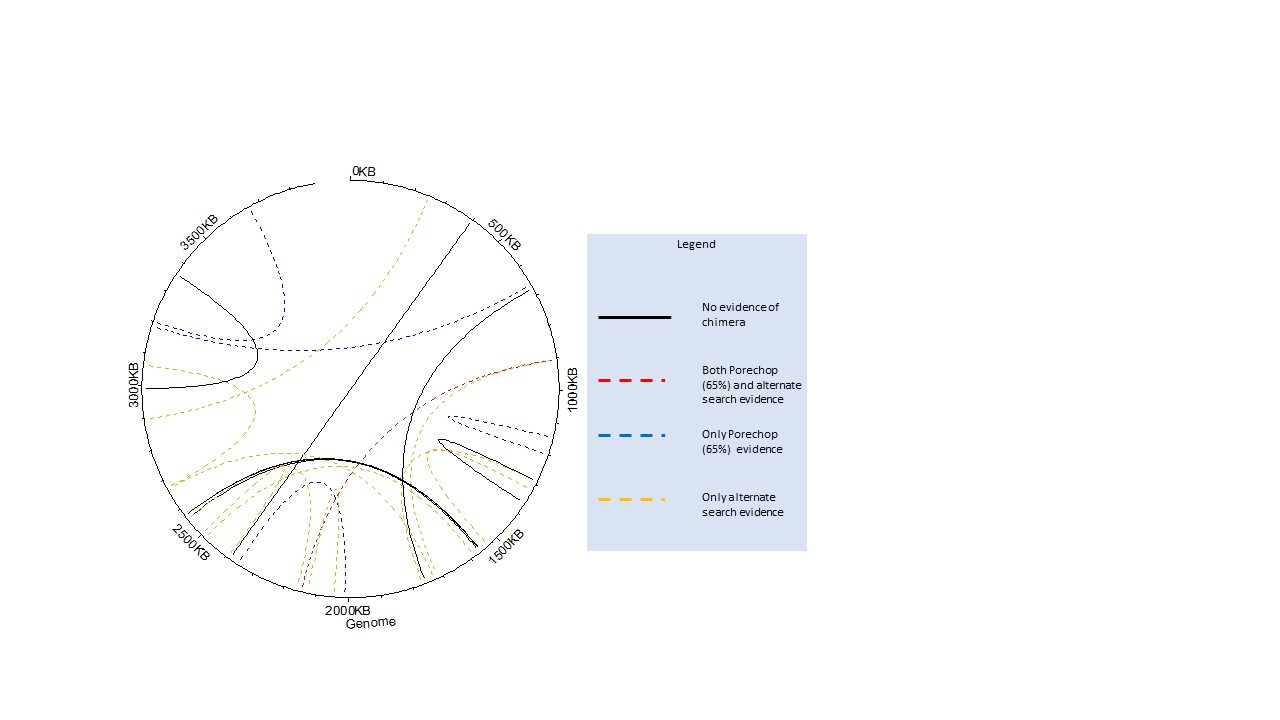
\includegraphics[width=\textwidth{}]{Chapter_2/baskey.jpg}
\caption{ Reads plotted in a Circos plot. Each read was categorised into 4 categories:Alterantive adapter search .}
\label{fig:Heatmap}
\end{figure}

Searching for adapters in this set of reads using Biostrings resulted in 17 of the 29 reads containing adapter sequences at the junction point. This was vastly more chimeric reads than porechop detected (6) which is likely due to extra stringencies in porechop. By combining the Biostrings and Porechop results it was found that 20 out of the 29 reads contained evidence from either search that there was an adapter sequence at the junction. In this specific applpication, high sensitivity was prioritised. It was more important to identify true positives, even at the cost of introducing false positives- I was searching for reads that had no evidence that they were contained adapter sequences at their junction. For this reason, if any credible match was found within 100bp of the junction (loosely defined as the ~3kb surrounding the repeat region in addition to the repeat)

\begin{figure}[h!]
\centering
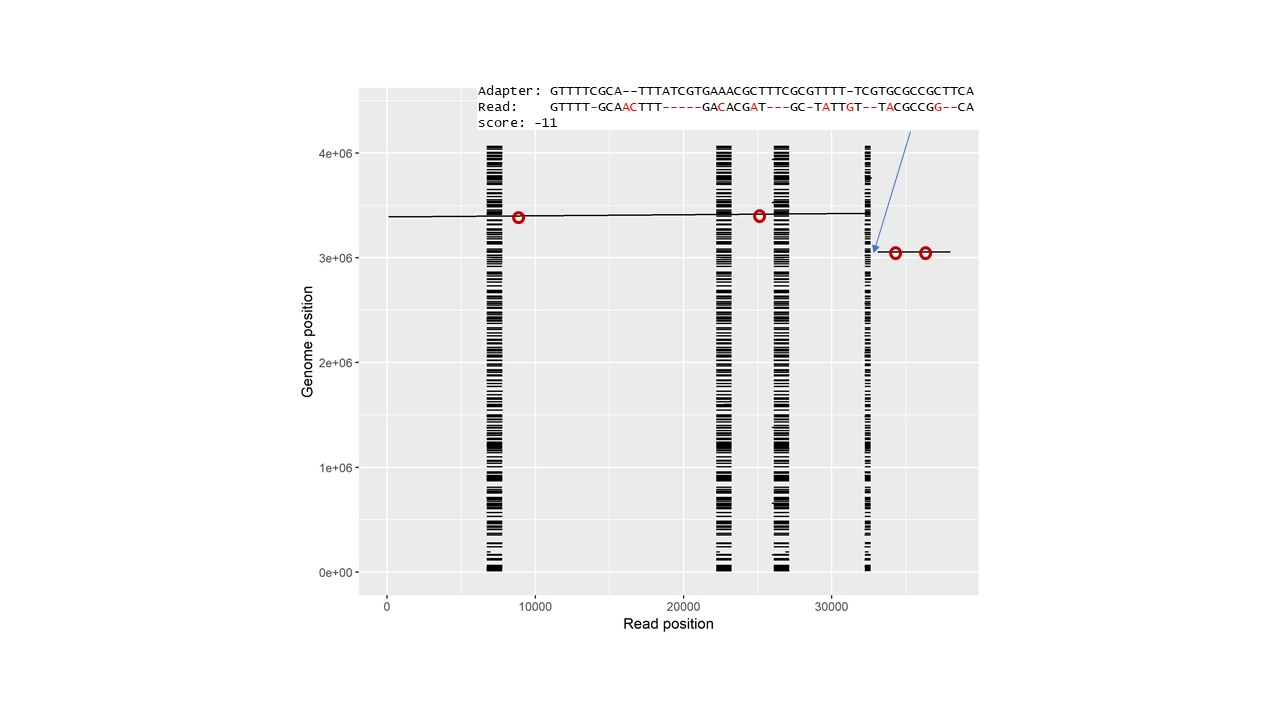
\includegraphics[width=\textwidth{}]{Chapter_2/Adapter read1 with FP.jpg}
\caption{ A read highlighted in the analysis that showed the most degraded adapter sequence found in an sequence gap, the alignment is shown and differences in the found adapter to the true adapter are in red lettering. The adapter was also found at other sites in the read, but these appear to be false positives as they had high homology to the reference BP sequence (circled in red).}
\label{fig:Heatmap}
\end{figure}


\begin{figure}[h!]
\centering
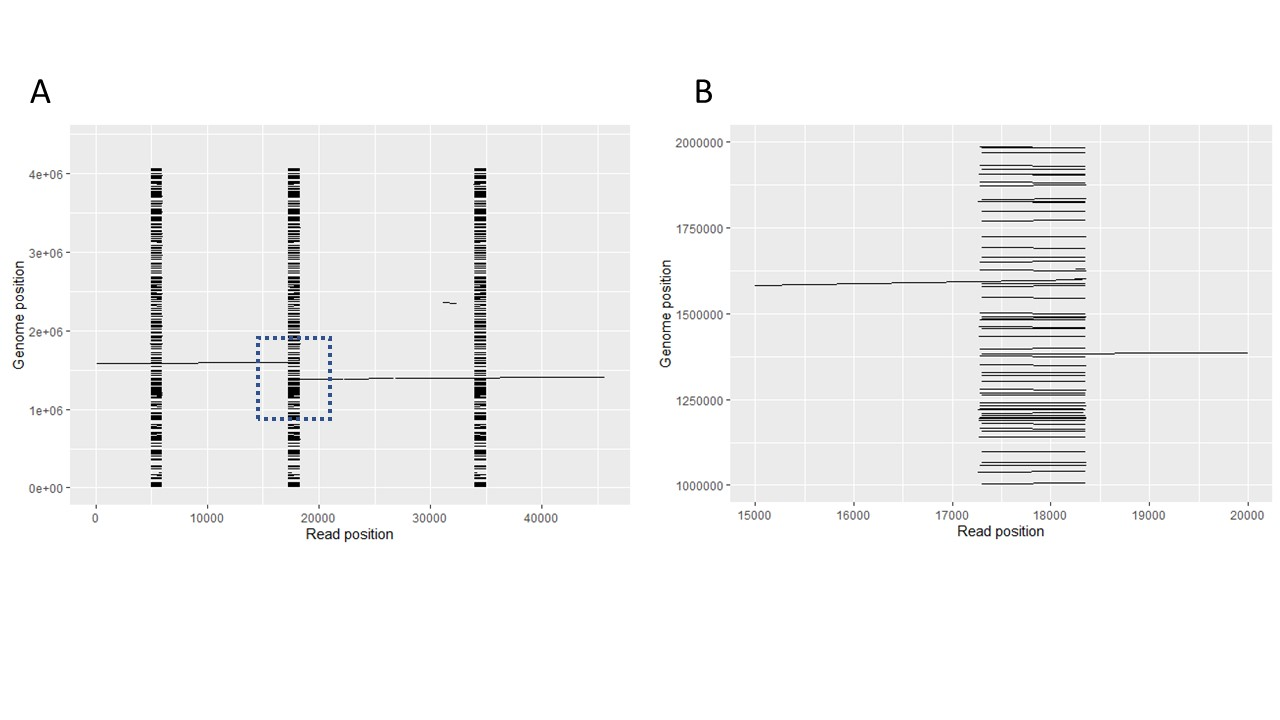
\includegraphics[width=\textwidth{}]{Chapter_2/Read 9(2).jpg}
\caption{ A read highlighted in the analysis that showed no evidence of being a chimera. The full read was blasted against the consensus sequence and all results were plotted(A). On closer examination of the blast results (1Mb-2Mb on the genome and 10kb-15kb on the read) (B) around the junction region, it can be seen that there are no gaps in homology and that the junction occurs in an insertion sequence (as the ~1kb sequence on the x axis occurs repeatedly on the 1Mb Y axis. This is a read that displays no hallmarks of a chimera.}
\label{fig:Heatmap}
\end{figure}

It is logical that the presence of an adapter, whether present as a recognisable sequence or not (or even if only partially present), would not map to the B.pertussis genome and therefore such gaps in sequence alignment can be exploited to identify probable chimeras. In support of this, of the 20 reads with recognisable adapters, 17 (85\%) contained gaps in sequence where the adapter was found. Not all gaps in a homology search between the reference genome and a read are expected to be chimeras as pores often experience a temporary drop in quality, leading to `glitched' stretches of DNA sequence that bear little resemblance to the true sequence. In this case, however, there is a strong link between adapter presence and gaps in sequence. An adapter can be present but not cause a gap in sequence if it is highly degraded. This was likely the case with the three reads which did not have gaps in homology. Of these three reads two had adapters recognised by porechop alone (which was demonstrated here to be unreliable for finding adapters) and one read had a degraded upstream adapter sequence present.


 Following this, it could be identified that out of the 9 reads which had no recognisable adapters, 33\%  of reads (3/9) had such gaps. 

\begin{figure}[h!]
\centering
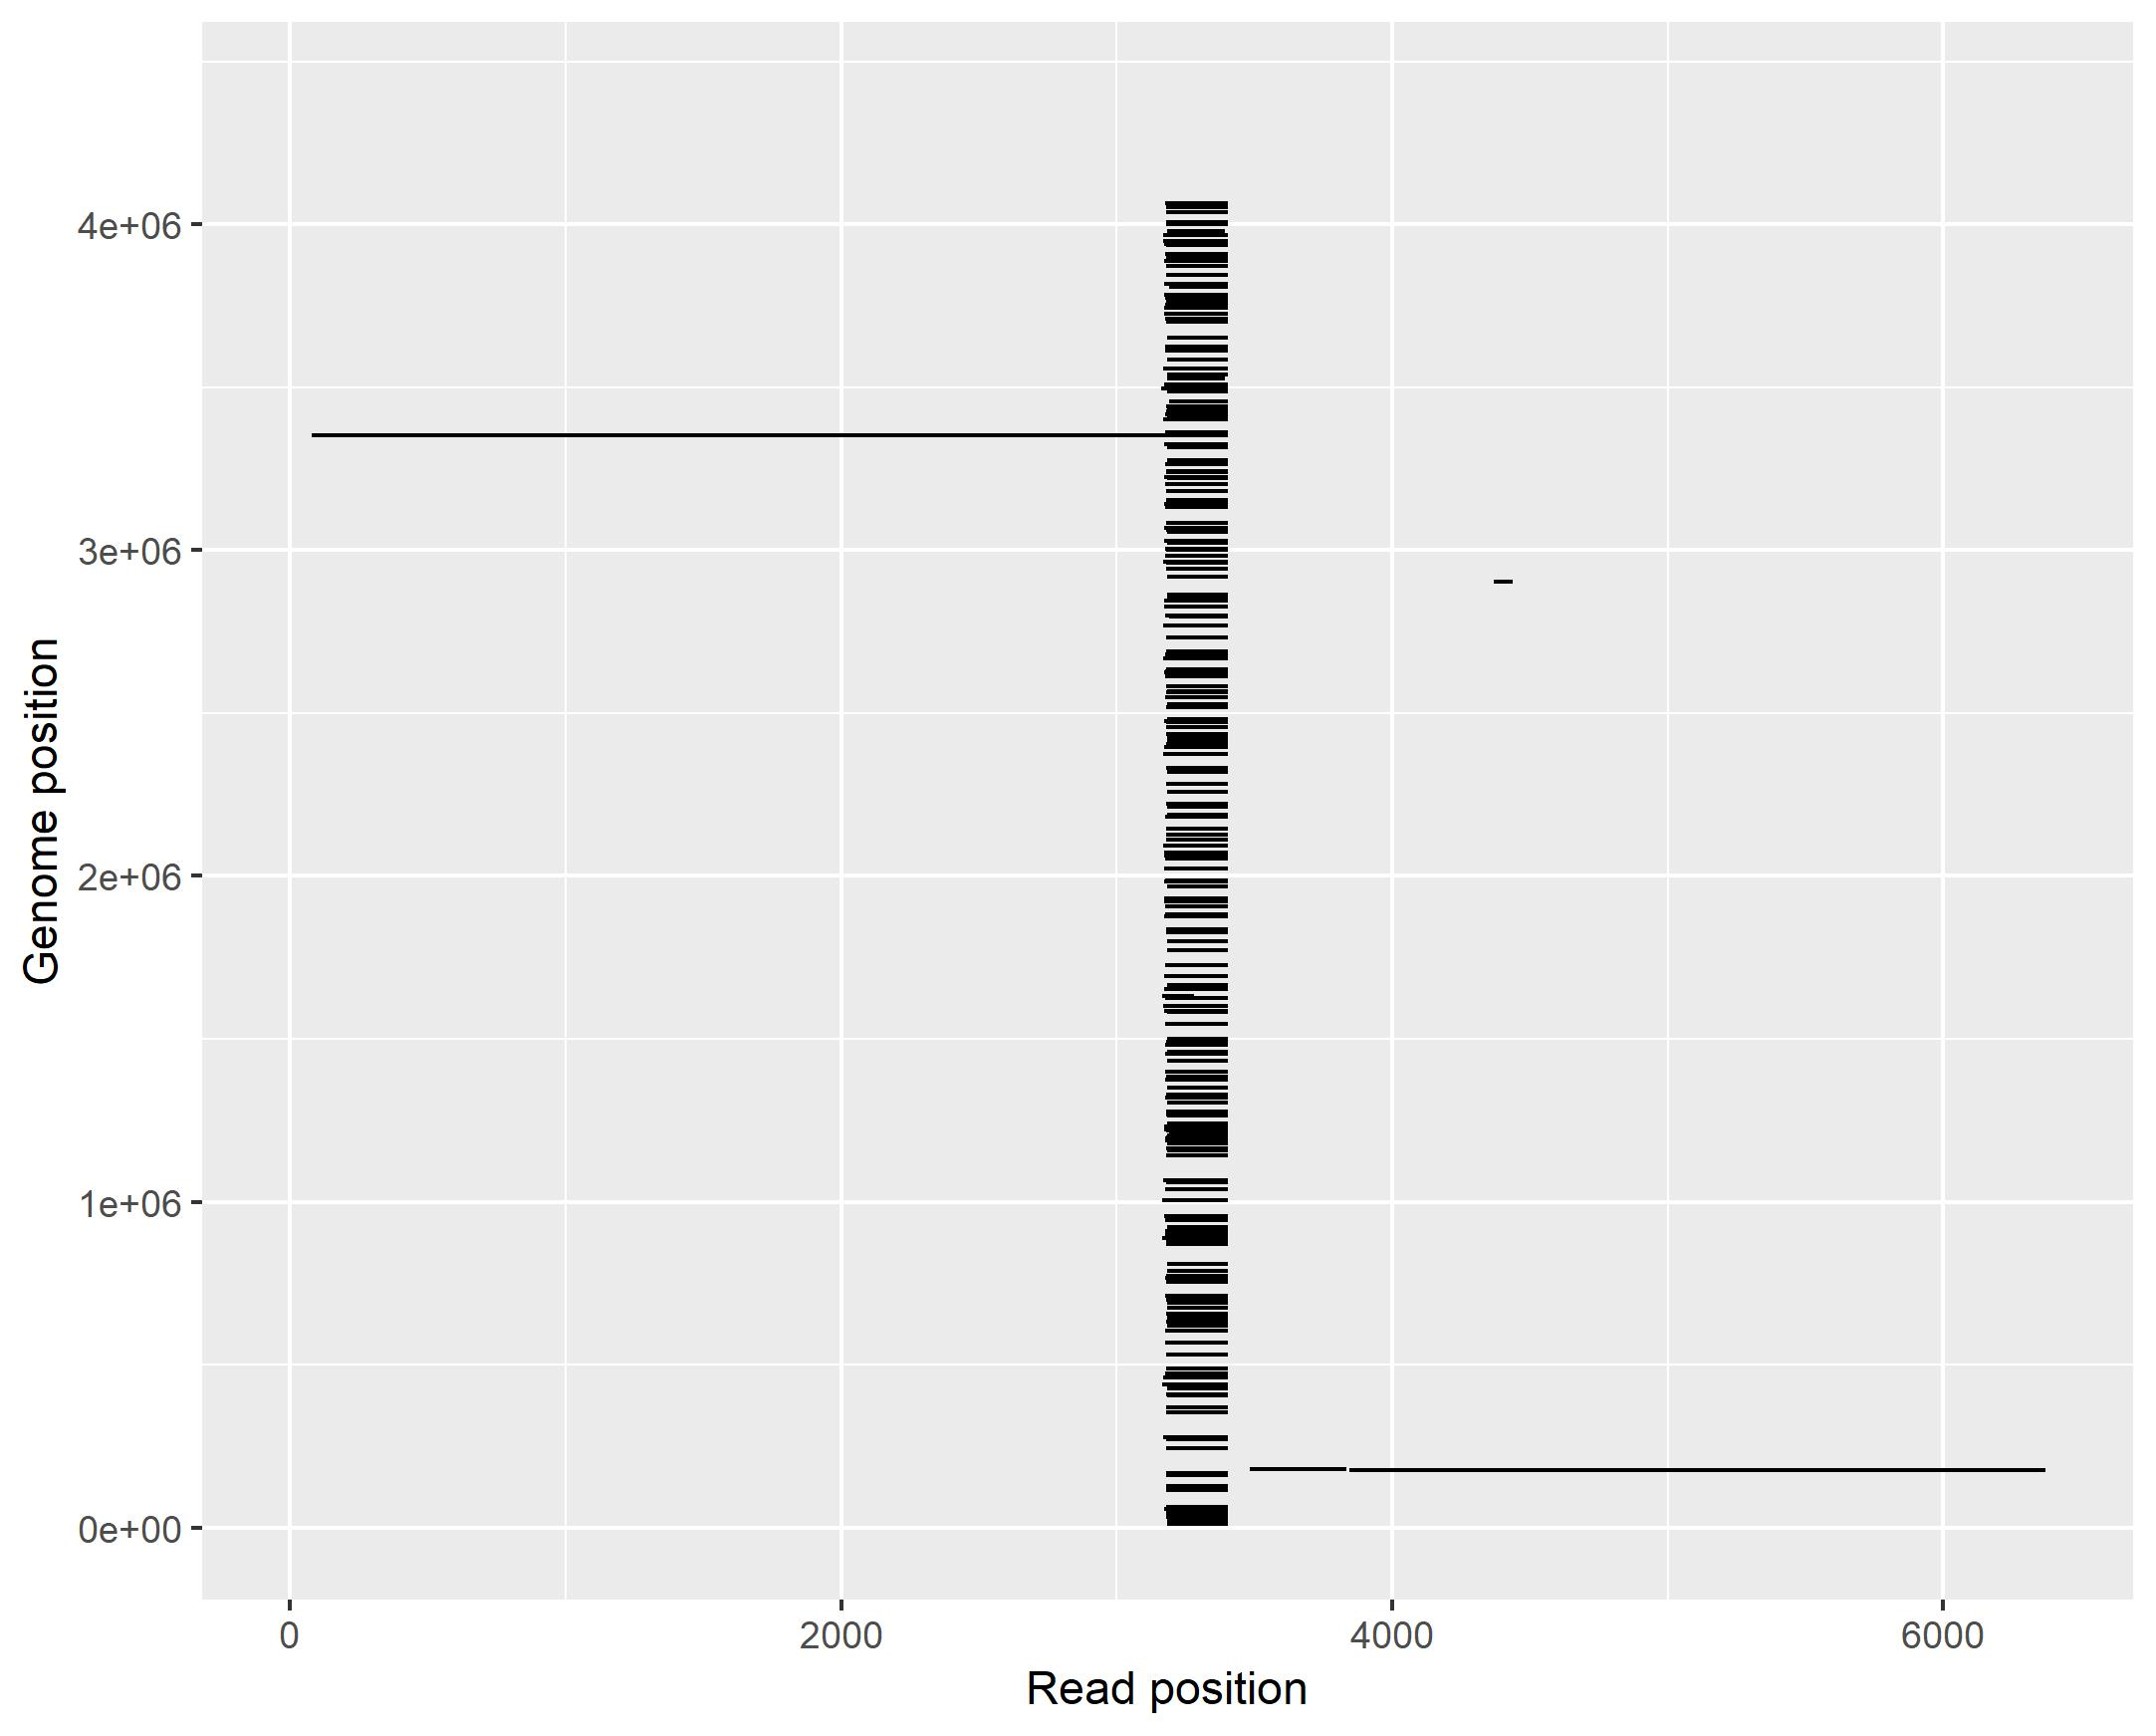
\includegraphics[width=\textwidth{}]{Chapter_2/Blast_results_347395.jpeg}
\caption{ Read with sequence gap which was highly correlated with adapter sequences. This read was identified by Biostrings to have an adapter but not by Porechop}
\label{fig:UK54_new_basket}
\end{figure}



\begin{figure}[h!]
\centering
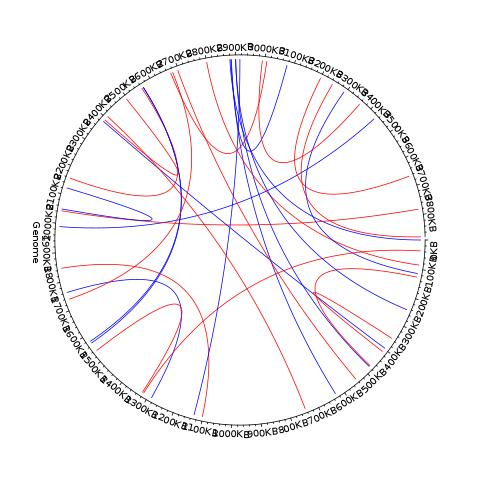
\includegraphics[width=\textwidth{}]{Chapter_2/UK54_new_basketball.jpeg}
\caption{  }
\label{fig:UK54_new_basket}
\end{figure}

It can therefore be concluded that of 29 reads identified by this analysis that there was no evidence that 8 were chimeras;indirect evidence that 4 were chimeras and direct evidence that 17 were chimeras.
Y reads had no gaps in sequence homology or any detectable adapter sequences at the junction
In conclusion, this in-depth disection of reads highlighted...


nanopore reads which revealed that genome-wide SV in bordetella pertussis could be observed by Nanopore sequencing. 

%The alignment scoring scheme used in this and subsequent alignments can be modified using the --scoring_scheme option (default: match = 3, mismatch = -6, gap open = -5, gap extend = -2).

%Plan: 

%First fig: actual basketballls 
\subsubsection{Weird reads}

%Put in two more reads here. 
\begin{figure}[h!]
\centering
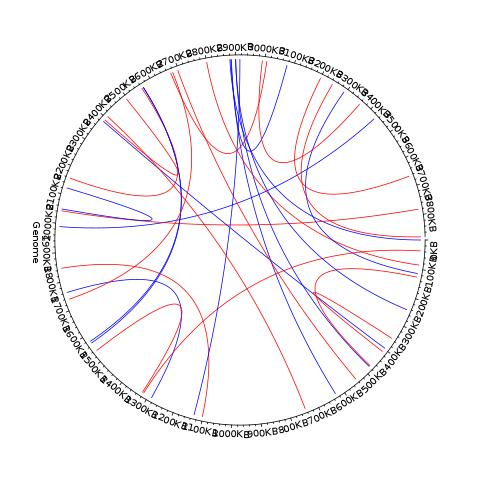
\includegraphics[width=\textwidth{}]{Chapter_2/UK54_new_basketball.jpeg}
\caption{  }
\label{fig:UK54_new_basket}
\end{figure}
 
 Manual inspection of these reads
 Figures XYZ show three of these reads, each representing the three of the different classes of reads from this analysis: Reads which appear to contain true SV's; reads with a probable adapter sequence at the junction and reads which contain a probable adapter sequence, but not at the junction.

%Reads
\subsubsection{Basketball insight}
When the pipeline was run with an adapter threshold of 64\% there were 25\% (~176,000) reads being detected as chimeras and split in the whole dataset. This data was intensely analysed (above) and any read that was produced by the pipline was also analysed by manual inspection.  The basketball plot to be limited to just X reads, each of which displayed no evidence of being a chimera.




\begin{figure}[h!]
\centering
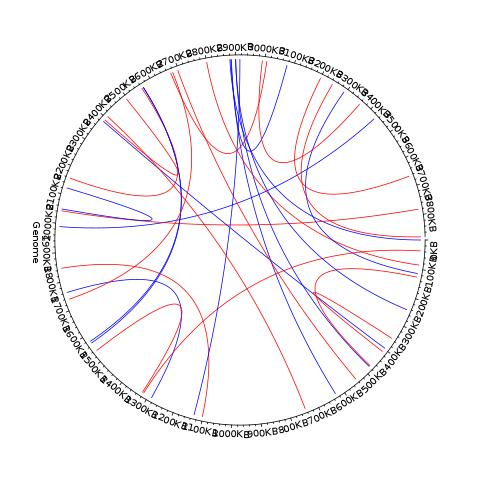
\includegraphics[width=\textwidth{}]{Chapter_2/UK54_new_basketball.jpeg}
\caption{  }
\label{fig:UK54_new_basket}
\end{figure}

